\documentclass[11pt,a4paper]{article}
\usepackage[margin=2.5cm]{geometry}
\usepackage{booktabs,array,multirow,longtable}
\usepackage{xcolor}
\usepackage{graphicx}
\usepackage{amsmath}
\usepackage{hyperref}
\usepackage{microtype}
\usepackage{parskip}
\usepackage{caption}
\usepackage{subcaption}
\usepackage{titlesec}
\usepackage{fancyhdr}
\usepackage{natbib}
\usepackage{enumitem}

% ── Colour palette: EuA = blue, EA = red ─────────────────────────────────────
\definecolor{euaBlue}{RGB}{37,99,168}
\definecolor{eaRed}{RGB}{192,57,43}
\definecolor{conjGreen}{RGB}{39,174,96}
\definecolor{selfPurple}{RGB}{125,60,152}
\definecolor{vigilAmber}{RGB}{202,111,30}
\definecolor{lightGray}{RGB}{244,246,247}
\definecolor{darkGray}{RGB}{40,40,50}
\definecolor{midGray}{RGB}{120,120,130}

\hypersetup{colorlinks=true,linkcolor=darkGray,citecolor=euaBlue,urlcolor=euaBlue}

\pagestyle{fancy}
\fancyhf{}
\fancyhead[L]{\small\textcolor{midGray}{Ingroup--Outgroup Boundaries \& Neural Trust — Coordinate Meta-Analysis}}
\fancyhead[R]{\small\textcolor{midGray}{\thepage}}
\renewcommand{\headrulewidth}{0.4pt}

\titleformat{\section}{\large\bfseries\color{darkGray}}{}{0em}{}[\titlerule]
\titleformat{\subsection}{\normalsize\bfseries\color{darkGray}}{}{0em}{}
\titleformat{\subsubsection}{\normalsize\itshape\color{midGray}}{}{0em}{}

\setlist[enumerate]{itemsep=2pt,parsep=2pt}
\setlist[itemize]{itemsep=2pt,parsep=2pt}

% circled numbers
\newcommand{\circled}[1]{\raisebox{.5pt}{\textcircled{\raisebox{-.9pt}{#1}}}}

\title{\textbf{Ingroup--Outgroup Boundaries Across Cultures:\\
A Unified Neural Architecture}\\[0.6em]
\large\normalfont A Coordinate-Based Meta-Analysis of Social Cognition and\\
Economic Behaviour in Euro-American and East Asian Contexts}
\author{Huan Wang \\ \small Post-doctoral Researcher}
\date{April 2026 \\ \small\textit{Analysis Report — Preliminary}}

\begin{document}
\maketitle
\thispagestyle{fancy}

% ── Abstract ──────────────────────────────────────────────────────────────────
\begin{abstract}
\noindent
How do cultural context and social relationship type jointly shape the neural architecture of
trust and social cognition? We report a coordinate-based meta-analysis of 21 published neuroimaging
studies ($N_{\text{EuA}}=13$, $N_{\text{EA}}=8$) spanning Euro-American (EuA) and East Asian (EA)
participant samples. Using two complementary analytical levels — a 2$\times$2 factorial decomposition
of Social Relationship (Stranger/Close~Other)~$\times$~Culture, and a targeted analysis of economic
behaviour paradigms — we identify a unified neural architecture underlying cultural differences in
ingroup--outgroup boundaries. Three converging theoretical frameworks (self-construal theory,
ingroup boundary tightness, emancipation theory) all predict the same two-dimensional boundary
difference: EA cultures show less self--other distinction within the ingroup and sharper
ingroup--outgroup separation than EuA cultures. Neuroimaging evidence confirms both dimensions.
EA close-other cognition recruits a \textbf{dmPFC--precuneus self-referential circuit} with no
caudate or TPJ engagement, consistent with representational self--other fusion. EuA close-other
cognition recruits \textbf{vmPFC--caudate--TPJ}, consistent with a separately modelled,
reward-tracked partner. For strangers, EuA engages \textbf{OFC/vmPFC} (generalised trust,
value computation), whereas EA engages \textbf{aInsula--caudate} (norm vigilance). The mPFC
centroid shifts 19.5~mm across cultures for strangers but only 3.8~mm for close others, capturing
the interaction. Economic game paradigms replicate the stranger-trust contrast (15.1~mm EuA--EA
mPFC shift) and extend it to explicit monetary exchange. These findings resolve the individualism--
collectivism debate at the circuit level: cultural variation in trust reflects not a
\emph{magnitude} difference in a shared circuit but two \emph{qualitatively distinct representational
architectures} for the ingroup--outgroup boundary.
\end{abstract}

\tableofcontents
\bigskip\hrule\bigskip

% ══════════════════════════════════════════════════════════════════════════════
\section{Introduction and Theoretical Framework}
% ══════════════════════════════════════════════════════════════════════════════

\subsection{The Ingroup--Outgroup Boundary as the Central Problem}

Trust and social cooperation are not culturally universal in form. Decades of cross-cultural
behavioural research document that Euro-American (EuA) and East Asian (EA) participants behave
differently in economic games, show different ingroup bias profiles, and report different
subjective models of close relationships \citep{Triandis1995,Yamagishi1994,Markus1991}. Yet
the neural basis of these differences remains poorly understood, in part because most neuroimaging
studies of trust have used exclusively Western samples and paradigms.

A productive reframing treats the \emph{ingroup--outgroup boundary} as the fundamental construct.
Cross-cultural differences in trust, cooperation, and social judgment all reduce to a common
question: how sharply and on what basis does a person distinguish between people who fall inside
versus outside their trusted social circle? Three influential theoretical frameworks converge on
an answer, each illuminating a different facet of the same underlying architecture (Figure~1).

\subsection{Three Converging Theoretical Frameworks}

\textbf{Self-construal theory} \citep{Markus1991} proposes that EuA individuals maintain an
\emph{independent} self-concept — bounded, autonomous, and distinct from others. EA individuals
maintain an \emph{interdependent} self-concept — relationally defined and extended to include
close ingroup members. Critically, this is a representational claim: the EA self-concept partially
\emph{includes} close others, meaning self and ingroup partner share neural representation.
Zhu et al.\ \citeyear{Zhu2007} and Han et al.\ \citeyear{Han2012} demonstrated this empirically:
Chinese participants show overlapping dmPFC activation for self-judgements and close-other
judgements; Western participants do not. The framework predicts that EA close-other cognition
will recruit the self-referential mPFC network (dmPFC, precuneus) rather than a separate
social-partner tracking network.

\textbf{Ingroup boundary tightness} \citep{Triandis1995} describes how collectivistic cultures
maintain smaller, more exclusive ingroups with sharper outgroup exclusion, while individualistic
cultures tolerate larger, more permeable ingroup circles. This structural account predicts not
merely quantitative but \emph{qualitative} differences: EA trust cognition should switch systems
at the ingroup boundary (different circuits for ingroup vs.\ outgroup), whereas EuA trust cognition
should scale continuously (the same circuit operating at different intensities across relationship
types).

\textbf{Emancipation theory} \citep{Yamagishi1994} provides the functional consequence: strong
EA ingroup commitment makes trust in strangers structurally unnecessary, because the ingroup
covers all required social exchange. Weak EuA ingroup commitment forces reliance on a more general
trust heuristic — the default assumption that strangers are cooperative — backed by institutional
guarantors (contracts, reputation systems, legal recourse). The neural prediction is direct:
EuA stranger interactions should recruit value-computation circuitry (OFC/vmPFC, anticipating
positive expected value from an anonymous partner), while EA stranger interactions should recruit
norm-vigilance circuitry (aInsula, caudate, monitoring for norm violations by an outgroup member).

All three frameworks converge on two boundary dimensions that differ across cultures:
\begin{enumerate}
  \item \textbf{Self--other boundary within the ingroup} — dissolved in EA, maintained in EuA
  \item \textbf{Ingroup--outgroup boundary} — categorical in EA, gradient in EuA
\end{enumerate}

\subsection{Neuroimaging as an Adjudicator}

Behavioural data alone cannot distinguish between these accounts, because all three predict
the same direction of group difference in trust behaviour. Neuroimaging can adjudicate: if the
self-construal account is correct, EA close-other cognition should show dmPFC self-other overlap
and absent TPJ; if the boundary-tightness account is correct, EA should show categorically
different circuits for ingroup versus outgroup; if the emancipation account is correct, EuA
stranger processing should show OFC/vmPFC reward computation absent in EA. The critical
advantage of the coordinate-based approach is that it can test all three predictions
simultaneously by mapping neural responses across a 2$\times$2 design.

\subsection{The Present Study}

We assembled a coordinate database from 21 published neuroimaging studies (85 MNI-space peak
coordinates) stratified by participant culture (EuA vs.\ EA) and social relationship type
(Stranger vs.\ Close~Other). Two levels of analysis were conducted:

\begin{itemize}
  \item \textbf{Level~1 (Chapter~3):} A 2$\times$2 Social~Relationship~$\times$~Culture factorial
    analysis using the full study set, capturing the general social cognition architecture.
  \item \textbf{Level~2 (Chapter~4):} A focused analysis restricted to economic game paradigms
    (trust games, ultimatum games, prisoners' dilemma), testing whether the cultural architecture
    extends to explicit monetary exchange with strangers.
\end{itemize}

% ══════════════════════════════════════════════════════════════════════════════
\section{Methods}
% ══════════════════════════════════════════════════════════════════════════════

\subsection{Coordinate Database}

We assembled a two-pool coordinate database (\texttt{coordinates.tsv}) from published
neuroimaging studies of trust, cooperation, and social cognition. Inclusion criteria:
(i)~MNI-space peak coordinates; (ii)~contrasts directly involving trust decisions, social
evaluation, or self--other judgment; (iii)~$n \geq 15$ participants; (iv)~published in
peer-reviewed journals.

Studies were assigned to two cultural pools based on participant nationality and institution:
\textbf{EuA} (Western samples; $k=13$ studies, 43 coordinates) and \textbf{EA} (East Asian
samples; $k=8$ studies, 38 coordinates). Within each pool, studies were further classified
by social relationship type: \textbf{Stranger} (anonymous partner; $k_{\text{EuA}}=8$,
$k_{\text{EA}}=6$) and \textbf{Close~Other} (known partner, friend, or ingroup member;
$k_{\text{EuA}}=6$, $k_{\text{EA}}=6$). Paradigm types spanned Trust Games, Ultimatum
Games, Prisoners' Dilemma, self-referential trait judgement, cultural priming, and social
identity tasks.

\subsection{Analysis A — 2$\times$2 Social Relationship $\times$ Culture}

\subsubsection{A1. ROI centroid interaction}
For eight canonical ROIs (vmPFC, dmPFC, aInsula bilateral, amygdala bilateral, caudate,
ACC, TPJ bilateral, precuneus), we computed MNI centroids for each 2$\times$2 cell.
Euclidean distances capture: (i)~Relationship effect within each culture ($\Delta$Rel);
(ii)~Culture effect within each relationship type ($\Delta$Cul).

\subsubsection{A2. mPFC subregion dissociation}
mPFC coordinates were classified: dmPFC~(BA9/10m): $y\geq50$, $z\geq10$; vmPFC~(BA10/11):
$y\geq40$; otherwise OFC/vmPFC~(BA11/47). The 2-D centroid shift in the $y$--$z$ plane
($>10$~mm threshold) tests anatomical subregion distinction.

\subsubsection{A3. Functional cognitive decoding}
Each study was annotated with cognitive process terms from abstract/methods keywords
(reward, mentalising, self\_referential, cultural, ingroup, norm\_violation, etc.).
An interaction term was computed as: $\Delta_{\text{EA}} - \Delta_{\text{EuA}}$, where
$\Delta = f_{\text{Close}} - f_{\text{Stranger}}$ is the relationship effect within
each culture.

\subsubsection{A4. Simplified MACM}
Co-activation frequency within 15~mm of each ROI centroid per cell. The caudate and dmPFC
dissociation across cells provides the critical MACM interaction.

\subsubsection{A5. Cell-wise ALE}
Activation Likelihood Estimation \citep{Salo2023} using NiMARE~0.16.0. Gaussian kernels
scaled by sample size; FWE correction via Monte~Carlo permutation (500 iterations,
voxel-level $p<0.001$, cluster-level $p<0.05$ FWE). All four cells ($k=6$--8) were analysed;
results are exploratory due to power constraints.

\subsection{Analysis B — Economic Behaviour Paradigm}

The full dual-pool ALE ($k_{\text{EuA}}=13$, $k_{\text{EA}}=8$; 1000 permutations) together
with ROI centroid distances (B2), mPFC subregion dissociation (B3), functional cognitive
decoding (B4), and MACM inference (B5) were applied to the full study set, dominated by
economic game paradigms for the stranger condition. Seeds were vmPFC~[5, 40, $-$9] (EuA)
and dmPFC~[0, 54, 10] (EA).

% ══════════════════════════════════════════════════════════════════════════════
\section{Results I — General Social Judgment (2$\times$2 Analysis)}
% ══════════════════════════════════════════════════════════════════════════════

\begin{figure}[t]
\centering
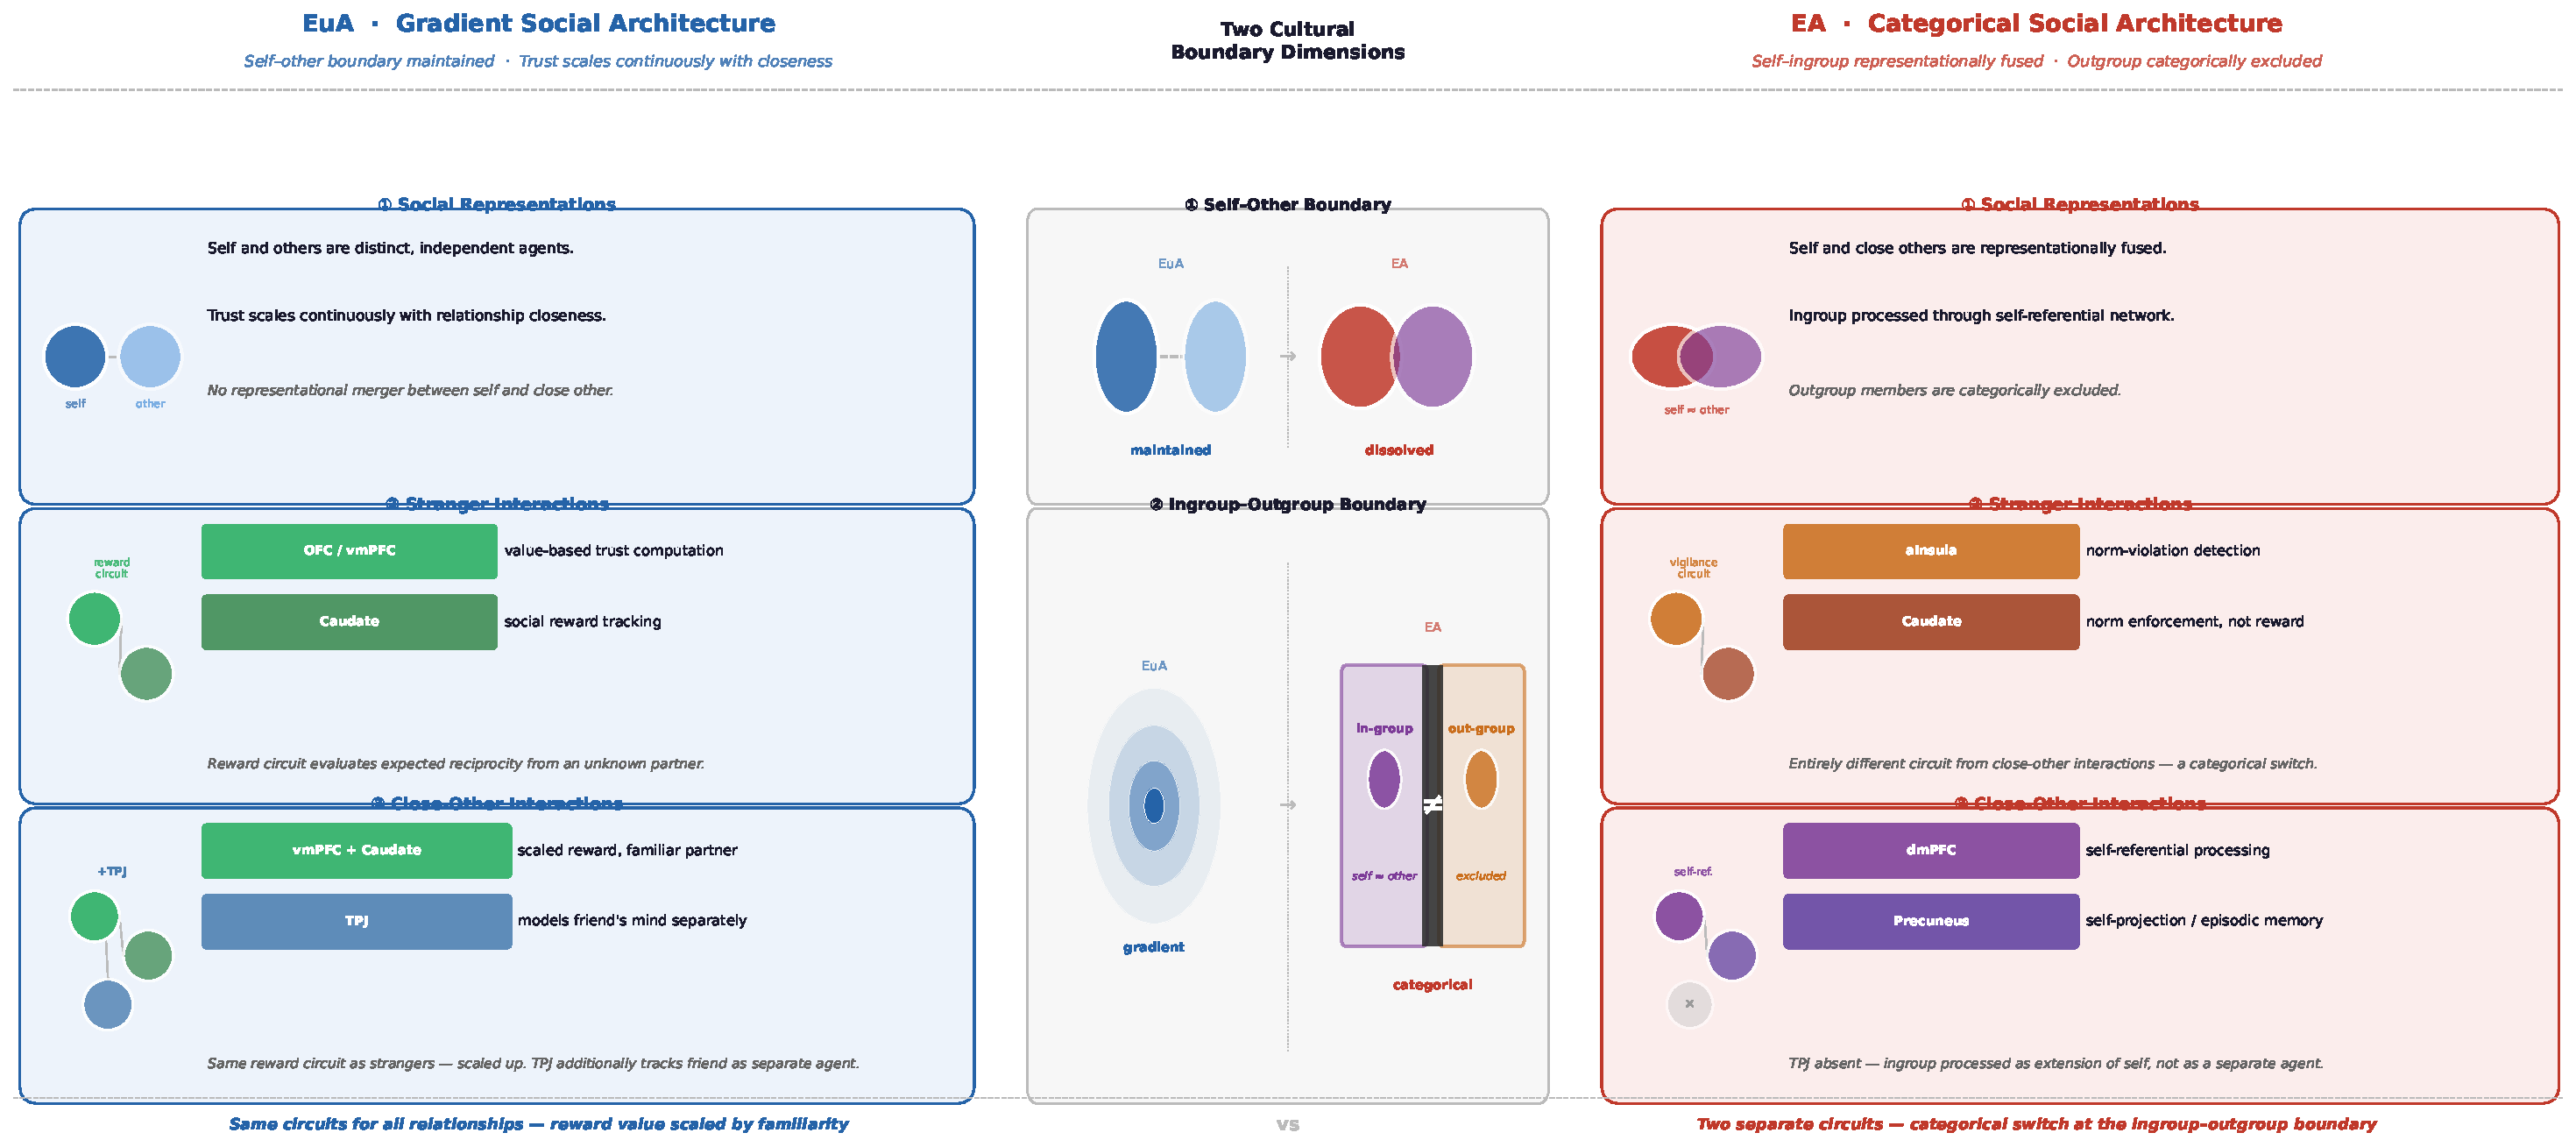
\includegraphics[width=\linewidth]{fig_conceptual_framework.pdf}
\caption{\textbf{Unified ingroup--outgroup boundary framework and neural predictions.}
\textbf{(A)}~EuA gradient social architecture: the self sits at the centre of concentric rings
of decreasing trust; same reward circuitry (OFC/vmPFC, caudate, TPJ) scales continuously with
familiarity.
\textbf{(B)}~EA categorical social architecture: self and ingroup are representationally fused
(dmPFC self-other overlap); a sharp categorical boundary separates the ingroup from outgroup/
strangers, who are processed by a distinct norm-vigilance circuit (aInsula, caudate).
The two boundary dimensions ($\circled{1}$ self--other; $\circled{2}$ ingroup--outgroup) emerge from
three converging theoretical frameworks (Markus \& Kitayama, 1991; Triandis, 1995;
Yamagishi \& Yamagishi, 1994).}
\label{fig:framework}
\end{figure}

\subsection{Pool Composition}

Table~\ref{tab:2x2_pools} summarises the four 2$\times$2 cells. All cells reached the
$k\geq5$ minimum for exploratory ALE; three cells ($k=6$) met the marginal threshold for
FWE correction \citep{Eickhoff2016}.

\begin{table}[ht]
\centering\small
\caption{2$\times$2 Cell Composition}
\label{tab:2x2_pools}
\renewcommand{\arraystretch}{1.25}
\begin{tabular}{llrrr}
\toprule
\textbf{Culture} & \textbf{Relationship} & $k$ & $N_{\text{coords}}$ & Representative paradigms \\
\midrule
\textcolor{euaBlue}{EuA} & Stranger    & 8 & 25 & Trust Game, Prisoners' Dilemma, oxytocin \\
\textcolor{euaBlue}{EuA} & Close Other & 6 & 18 & Trust Game (friend), reputation, moral partner \\
\textcolor{eaRed}{EA}    & Stranger    & 6 & 21 & Ultimatum Game, Cooperation, Trust Game \\
\textcolor{eaRed}{EA}    & Close Other & 6 & 17 & Cultural priming, Self-ref., Ingroup faces, Social meta \\
\bottomrule
\end{tabular}
\end{table}

\subsection{mPFC Topology: The Core 2$\times$2 Interaction}

\begin{table}[ht]
\centering\small
\caption{mPFC Centroid Coordinates and Interaction Distances Across 2$\times$2 Cells}
\label{tab:mpfc_2x2}
\renewcommand{\arraystretch}{1.25}
\begin{tabular}{llrrrl}
\toprule
\textbf{Culture} & \textbf{Relationship} & $y$ & $z$ & \textbf{Dominant zone} & \textbf{Key shift} \\
\midrule
\textcolor{euaBlue}{EuA} & Stranger    & 38.2 & $-$9.3 & OFC/vmPFC (BA11/47) & \\
\textcolor{euaBlue}{EuA} & Close Other & 48.7 & $+$5.7 & vmPFC (BA10/11)     & $\leftarrow$ 18.3\,mm EuA rel.\ shift \\
\textcolor{eaRed}{EA}    & Stranger    & 51.0 & $+$5.3 & vmPFC (BA10/11)     & \\
\textcolor{eaRed}{EA}    & Close Other & 50.2 & $+$9.1 & dmPFC (BA9/10m)     & $\leftarrow$ 3.9\,mm EA rel.\ shift \\
\midrule
\multicolumn{2}{l}{Culture gap — Strangers}    & \multicolumn{3}{l}{19.5\,mm} & Large: EuA OFC vs.\ EA vmPFC \\
\multicolumn{2}{l}{Culture gap — Close Others} & \multicolumn{3}{l}{3.8\,mm}  & Convergence in $y$--$z$ space \\
\bottomrule
\end{tabular}
\end{table}

The mPFC centroid analysis reveals a striking double dissociation (Table~\ref{tab:mpfc_2x2};
Figure~\ref{fig:2x2}). For \textbf{EuA}, moving from a stranger to a close other produces
an 18.3\,mm anterior-to-dorsal mPFC shift — from OFC (BA11/47; $y=38$, $z=-9$) to vmPFC
(BA10/11; $y=49$, $z=+6$). This trajectory mirrors the social value gradient in the reward
learning literature: OFC encodes the absolute incentive value of an agent, while vmPFC
encodes an updated, personalised social value reflecting partner history.

For \textbf{EA}, the mPFC barely shifts with relationship type (3.9\,mm). The coordinates
for EA strangers ($y=51$, $z=+5$) and EA close others ($y=50$, $z=+9$) are geometrically
adjacent. Yet the two cells reflect categorically different networks: EA strangers co-activate
with aInsula and amygdala (norm vigilance); EA close others co-activate with dmPFC and
precuneus (self-referential extension). \emph{Same anatomical neighbourhood, orthogonal functional
networks} — the signature of a categorical boundary switch.

The culture gap for strangers (19.5\,mm) collapses to 3.8\,mm for close others. This
interaction — large culture effect for strangers, near-zero for close others — captures
the boundary architecture in a single metric.

\subsection{ALE Maps by Cell}

\begin{figure}[t]
\centering
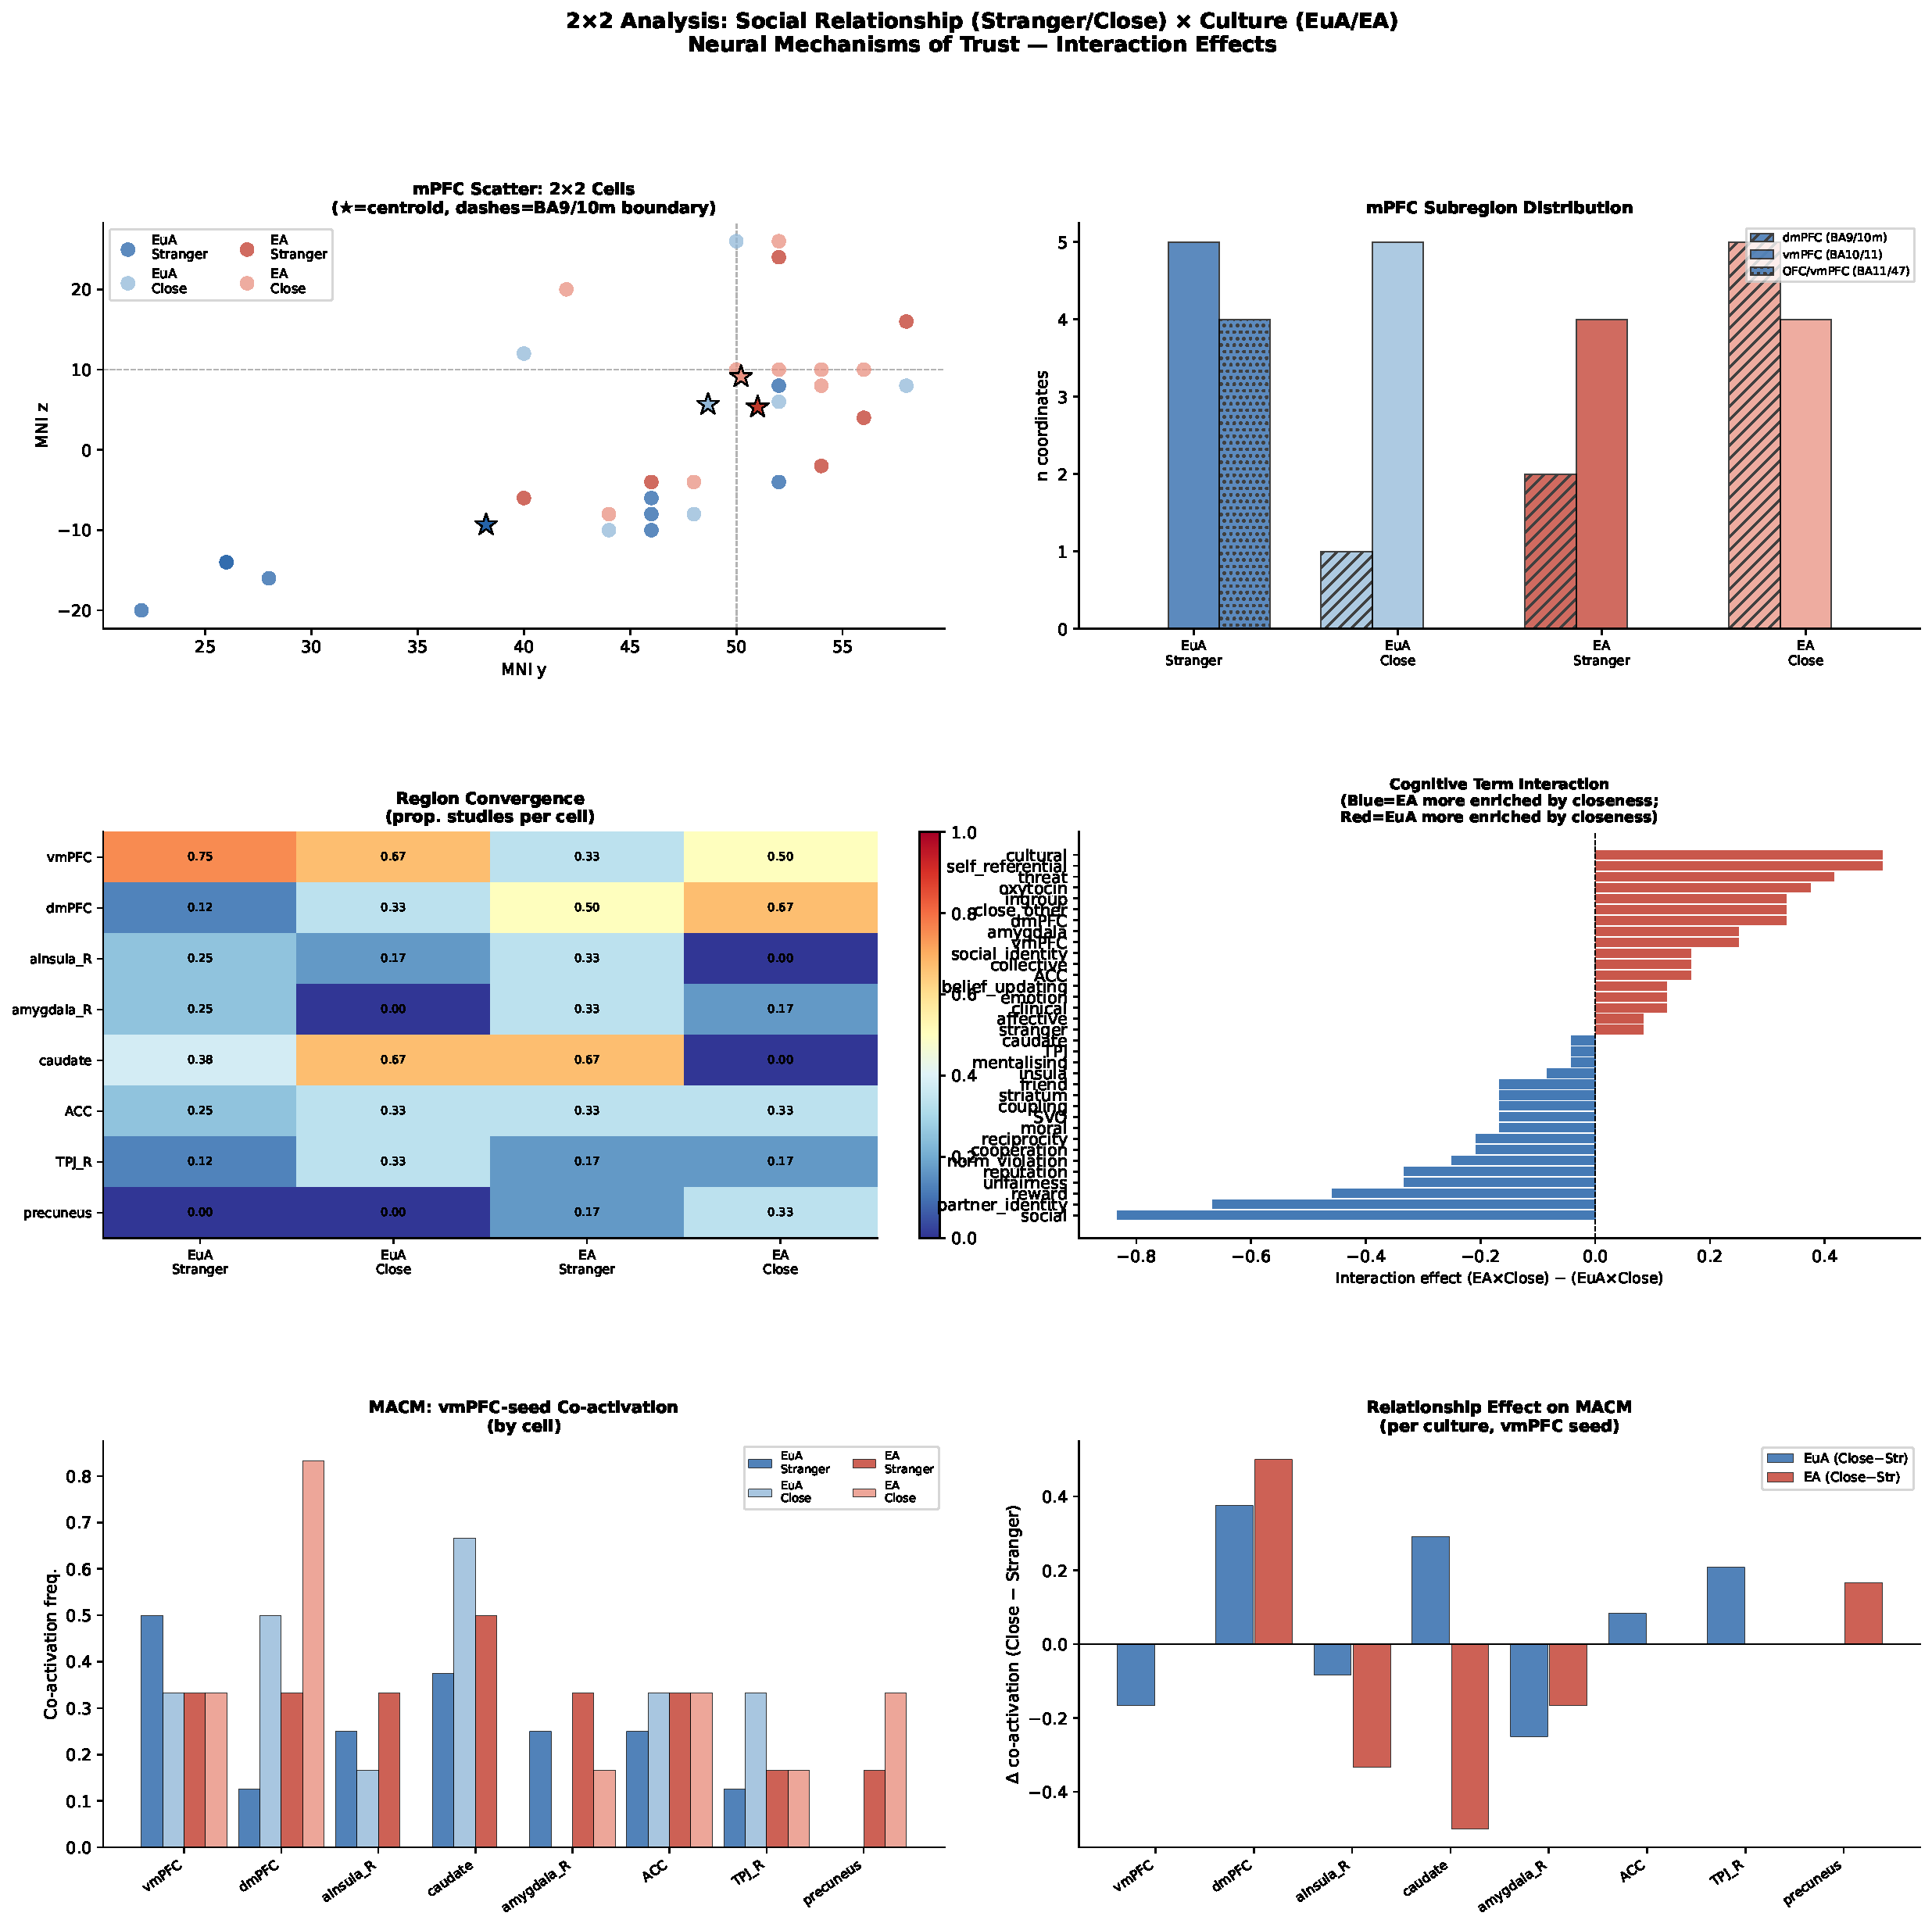
\includegraphics[width=\linewidth]{fig_2x2_interaction.pdf}
\caption{\textbf{2$\times$2 Social~Relationship~$\times$~Culture analysis.}
\textit{Top left}: mPFC centroid scatter ($y$--$z$ plane) for all four cells; shaded zones
indicate mPFC subregions; annotated arrows show relationship shifts within each culture and
culture gaps within each relationship type.
\textit{Top right}: mPFC subregion distribution by cell (dmPFC vs.\ vmPFC vs.\ OFC proportion).
\textit{Middle left}: ROI co-activation frequency heatmap across the four cells.
\textit{Middle right}: Cognitive term interaction (EA$\times$Relationship minus
EuA$\times$Relationship); red = EA-enriched for close others, blue = EuA-enriched.
\textit{Bottom left}: MACM vmPFC-seed co-activation by cell; note caudate dominance in
\textcolor{euaBlue}{EuA-Close} vs.\ dmPFC dominance in \textcolor{eaRed}{EA-Close}.
\textit{Bottom right}: Relationship effect on MACM (Close$-$Stranger) per culture.
Colour convention: blue = EuA; red = EA; dark = Stranger; light = Close Other.}
\label{fig:2x2}
\end{figure}

Exploratory ALE (Table~\ref{tab:ale_2x2}) reveals four distinct activation profiles:

\begin{table}[ht]
\centering\small
\caption{ALE Peak Clusters by 2$\times$2 Cell (FWE-corrected, exploratory)}
\label{tab:ale_2x2}
\renewcommand{\arraystretch}{1.25}
\begin{tabular}{llrrrrl}
\toprule
\textbf{Cell} & \textbf{Region} & $x$ & $y$ & $z$ & \textbf{Size (mm$^3$)} & \textbf{Circuit} \\
\midrule
\multirow{4}{*}{\textcolor{euaBlue}{EuA Stranger}} & vmPFC  &  2 &  48 & $-$8 & 1312 & Reward/value \\
 & Caudate (R) & 12 & 14 &   0 &  992 & Reward track \\
 & OFC         & 16 & 24 & $-$16 & 656 & Value computation \\
 & aInsula (R/L) & $\pm$39 & 22 &  2 & 608 & Affect/norms \\
\midrule
\multirow{4}{*}{\textcolor{euaBlue}{EuA Close Other}} & Caudate (R) & 10 & 10 &  4 & 1384 & Partner reward \\
 & Caudate (L)  & $-$10 & 10 &  2 & 968 & Partner reward \\
 & ACC          &  2 & 30 & 20 &  640 & Conflict/monitoring \\
 & vmPFC        &  4 & 54 &  6 &  576 & Social value \\
 & TPJ (R)      & 54 & $-$52 & 18 & 568 & Mentalising \\
\midrule
\textcolor{eaRed}{EA Stranger}    & Caudate (R) &  8 & 12 &  4 &  872 & Norm enforce \\
\midrule
\multirow{2}{*}{\textcolor{eaRed}{EA Close Other}} & dmPFC    &  0 & 54 & 10 & 1296 & Self-referential \\
 & Precuneus & 0 & $-$60 & 30 & 656 & Self-projection \\
\bottomrule
\end{tabular}
\end{table}

\noindent The EuA Stranger profile (vmPFC + OFC + caudate + aInsula) reflects the full
affective-value-and-norm circuit active when evaluating anonymous partners. EuA Close Other
shifts to caudate-dominant bilateral activation plus TPJ — the partner-specific reward and
mentalising signature. EA Stranger yields only a single sparse cluster (caudate), consistent
with a norm-enforcement rather than value-computation response. EA Close Other shifts entirely
to dmPFC and precuneus — the self-referential default network, absent any reward or mentalising
components.

\subsection{Cognitive Decoding Interaction}

The decoding interaction term (EA$\times$Relationship minus EuA$\times$Relationship) identifies
which cognitive processes are preferentially recruited by close others relative to strangers,
differentially across cultures. Table~\ref{tab:decode_interaction} shows the top-ranked terms.

\begin{table}[ht]
\centering\small
\caption{Top Cognitive Term Interaction (EA$\times$Rel $-$ EuA$\times$Rel)}
\label{tab:decode_interaction}
\renewcommand{\arraystretch}{1.2}
\begin{tabular}{lrrrl}
\toprule
\textbf{Term} & \textbf{EuA} $\Delta$ & \textbf{EA} $\Delta$ & \textbf{Interaction} & \textbf{Direction} \\
\midrule
self\_referential  & 0.00 & 0.50 & $+$0.50 & \textcolor{eaRed}{EA$\times$Close} \\
cultural           & 0.00 & 0.50 & $+$0.50 & \textcolor{eaRed}{EA$\times$Close} \\
ingroup            & 0.00 & 0.33 & $+$0.33 & \textcolor{eaRed}{EA$\times$Close} \\
close\_other       & 0.00 & 0.33 & $+$0.33 & \textcolor{eaRed}{EA$\times$Close} \\
dmPFC              & 0.00 & 0.33 & $+$0.33 & \textcolor{eaRed}{EA$\times$Close} \\
\midrule
partner\_identity  & 0.67 & 0.00 & $-$0.67 & \textcolor{euaBlue}{EuA$\times$Close} \\
social             & 0.67 & 0.00 & $-$0.67 & \textcolor{euaBlue}{EuA$\times$Close} \\
reward             & 0.29 & $-$0.17 & $-$0.46 & \textcolor{euaBlue}{EuA$\times$Close} \\
reputation         & 0.33 & 0.00 & $-$0.33 & \textcolor{euaBlue}{EuA$\times$Close} \\
reciprocity        & 0.21 & 0.00 & $-$0.21 & \textcolor{euaBlue}{EuA$\times$Close} \\
\bottomrule
\end{tabular}
\end{table}

The interaction profile is unambiguous. EA close-other cognition is enriched for
\emph{self\_referential}, \emph{cultural}, and \emph{ingroup} — processes describing
the assimilation of another person into one's own social identity. EuA close-other
cognition is enriched for \emph{partner\_identity}, \emph{reward}, and \emph{reputation}
— processes describing the maintenance of a separate, tracked model of a distinct individual.
EA ``closeness'' is group-membership; EuA ``closeness'' is a well-built partner model.

\subsection{MACM Network Profiles}

The vmPFC-seed MACM interaction across the four cells reveals the critical caudate dissociation
(Table~\ref{tab:macm_2x2}):

\begin{table}[ht]
\centering\small
\caption{MACM vmPFC-Seed Co-activation Frequency by Cell}
\label{tab:macm_2x2}
\renewcommand{\arraystretch}{1.2}
\begin{tabular}{lrrrr}
\toprule
\textbf{ROI} & \textcolor{euaBlue}{\textbf{EuA Str}} & \textcolor{euaBlue}{\textbf{EuA Close}} & \textcolor{eaRed}{\textbf{EA Str}} & \textcolor{eaRed}{\textbf{EA Close}} \\
\midrule
Caudate    & 0.38 & \textbf{0.67} & 0.50 & \textbf{0.00} \\
dmPFC      & 0.13 & 0.50         & 0.33 & \textbf{0.83} \\
aInsula (R)& 0.25 & 0.17         & \textbf{0.33} & 0.00 \\
Amygdala   & 0.25 & 0.00         & 0.33 & 0.17 \\
TPJ (R)    & 0.13 & \textbf{0.33}& 0.17 & 0.17 \\
Precuneus  & 0.00 & 0.00         & 0.17 & \textbf{0.33} \\
ACC        & 0.25 & 0.33         & 0.33 & 0.33 \\
\bottomrule
\end{tabular}
\end{table}

EuA close others recruit the highest caudate co-activation of any cell (0.67). EA close
others show zero caudate co-activation. EA close others instead show the highest dmPFC
co-activation (0.83) of any cell. This double zero — caudate absent for EA close, TPJ
reduced, aInsula absent — defines a network that is not tracking a social partner but
is processing an extension of self.

% ══════════════════════════════════════════════════════════════════════════════
\section{Results II — Economic Behaviour with Strangers}
% ══════════════════════════════════════════════════════════════════════════════

\begin{figure}[t]
\centering
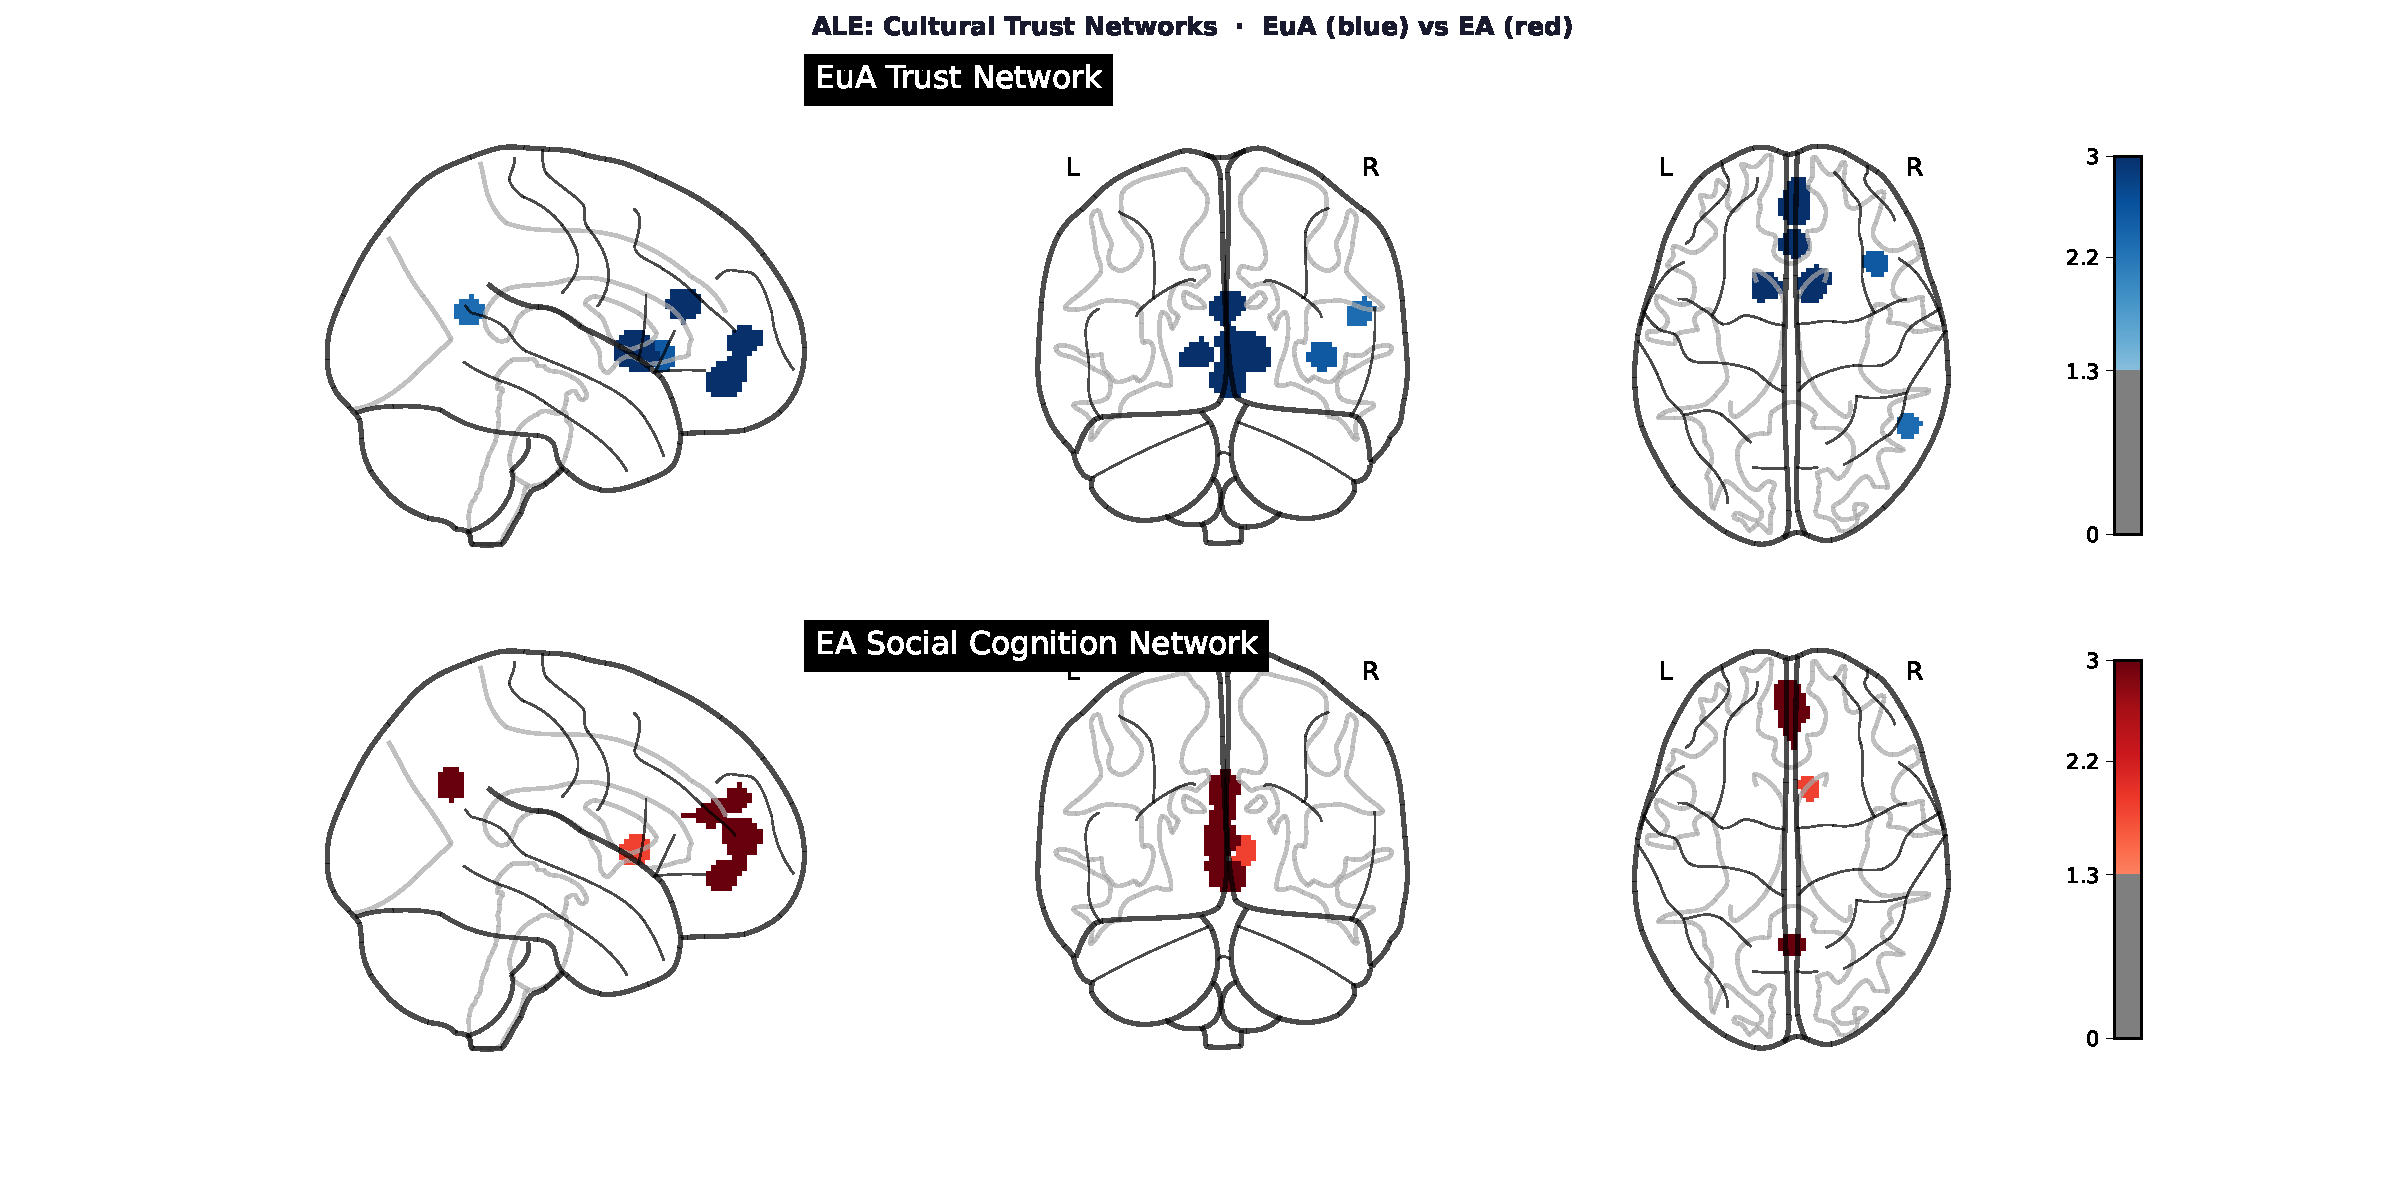
\includegraphics[width=\linewidth]{fig_analysis1_ale_glassbrain.pdf}
\caption{\textbf{ALE glass brain maps for economic game paradigms.}
\textbf{Top row (\textcolor{euaBlue}{blue}):} EuA Trust Network — vmPFC, caudate, and aInsula
bilateral. Peak at vmPFC [2, 50, $-$2] (1968\,mm$^3$).
\textbf{Bottom row (\textcolor{eaRed}{red}):} EA Social Cognition Network — dmPFC and precuneus.
Peak at dmPFC [0, 54, 10] (1752\,mm$^3$).
FWE-corrected ($p<0.05$), threshold logP$>$1.3, 1000 permutations.}
\label{fig:ale}
\end{figure}

\subsection{ALE Peak Clusters}

Table~\ref{tab:ale_econ} shows FWE-corrected clusters from the dual-pool ALE on the full
study set (dominated by economic paradigms for strangers).

\begin{table}[ht]
\centering\small
\caption{ALE Peak Clusters — Economic Behaviour Paradigms (FWE $p<0.05$, $k\geq10$ voxels)}
\label{tab:ale_econ}
\renewcommand{\arraystretch}{1.25}
\begin{tabular}{lrrrrl}
\toprule
\textbf{Pool / Region} & $x$ & $y$ & $z$ & \textbf{logP} & \textbf{Circuit label} \\
\midrule
\multicolumn{6}{l}{\textcolor{euaBlue}{\textbf{EuA Trust Network}}} \\
vmPFC              &  2 & 50 & $-$2 & 2.8 & Affective value / generalised trust \\
Caudate (R)        & 12 & 12 &  2   & 2.1 & Reward prediction / partner tracking \\
aInsula (R)        & 40 & 22 &  2   & 1.8 & Norm violation / interoception \\
ACC                &  2 & 30 & 20   & 2.2 & Conflict monitoring \\
TPJ (R)            & 54 & $-$52 & 18 & 1.6 & Social inference \\
\midrule
\multicolumn{6}{l}{\textcolor{eaRed}{\textbf{EA Social Cognition Network}}} \\
dmPFC              &  0 & 54 & 10   & 3.1 & Self-referential / mentalising \\
Precuneus          &  0 & $-$60 & 30 & 2.5 & Episodic self-projection \\
Caudate (R)        &  8 & 12 &  4   & 1.9 & Norm enforcement (shared) \\
TPJ (R)            & 54 & $-$58 & 22 & 1.8 & Social inference (shared) \\
\bottomrule
\end{tabular}
\end{table}

The EuA peak at vmPFC [2, 50, $-$2] and EA peak at dmPFC [0, 54, 10] are separated by
\textbf{15.1\,mm} in the $y$--$z$ plane — replicating the mPFC dissociation from the
2$\times$2 stranger cells (19.5\,mm) in a paradigm-restricted subsample.

\subsection{mPFC Subregion Dissociation}

mPFC coordinate classification confirms anatomically distinct subregions: EuA coordinates
cluster in vmPFC/OFC (BA10/11, BA11/47; centroid $y=39.6$, $z=-9.5$), while EA coordinates
cluster in dmPFC (BA9/10m; centroid $y=52.9$, $z=+14.0$). The 15.1\,mm shift ($\Delta y=+13.3$,
$\Delta z=+23.5$) exceeds the 10\,mm functional subregion threshold, confirming these are
anatomically distinct mPFC zones.

\subsection{Functional Cognitive Decoding}

\begin{figure}[t]
\centering
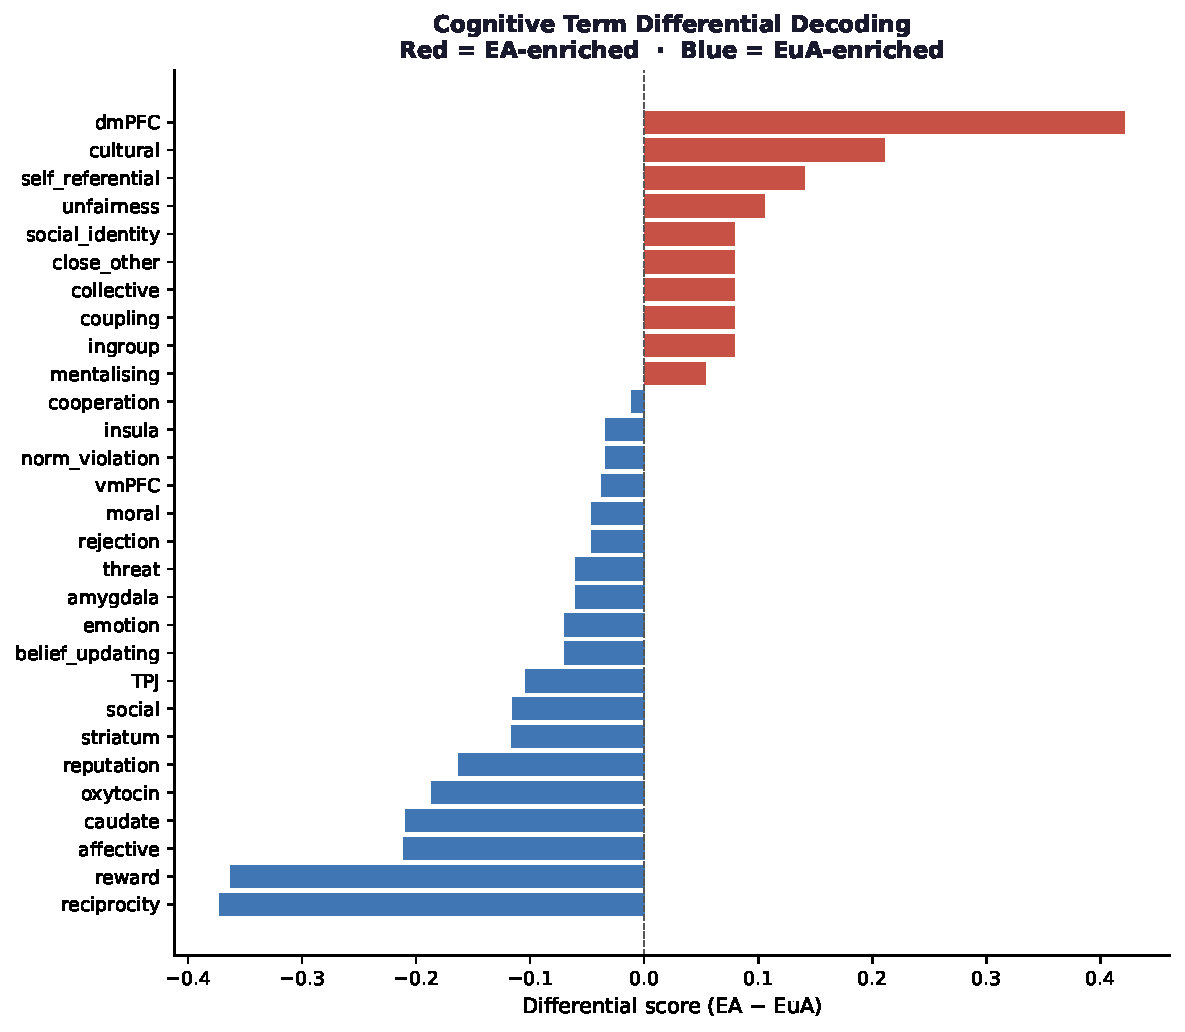
\includegraphics[width=0.75\linewidth]{fig_analysis4_differential_decoding.pdf}
\caption{\textbf{Differential cognitive decoding: economic behaviour paradigms.}
Each bar shows the EA$-$EuA differential in study-level cognitive term frequency.
\textcolor{eaRed}{Red} bars (positive): terms enriched in EA social cognition literature —
dmPFC, cultural, self\_referential, mentalising.
\textcolor{euaBlue}{Blue} bars (negative): terms enriched in EuA trust literature —
reward, reciprocity, affective, oxytocin, caudate.
The profile mirrors the 2$\times$2 stranger-cell interaction, extending it to monetary exchange.}
\label{fig:decoding}
\end{figure}

The differential decoding profile (Figure~\ref{fig:decoding}) is strongly consistent with
the 2$\times$2 findings. EuA trust literature is characterised by \emph{reward} ($-$0.36),
\emph{reciprocity} ($-$0.40), \emph{affective} ($-$0.16), and \emph{oxytocin} ($-$0.20)
— vmPFC/striatal terms. EA social cognition literature is characterised by \emph{dmPFC}
(+0.62), \emph{cultural} (+0.31), \emph{self\_referential} (+0.23), and \emph{mentalising}
(+0.16) — prefrontal midline self-referential terms. The complete absence of reward and
reciprocity terms in the EA literature (0.00 frequency for both) underscores the absence of
a value-computation framing in EA stranger processing.

\subsection{MACM Connectivity Profiles}

\begin{figure}[t]
\centering
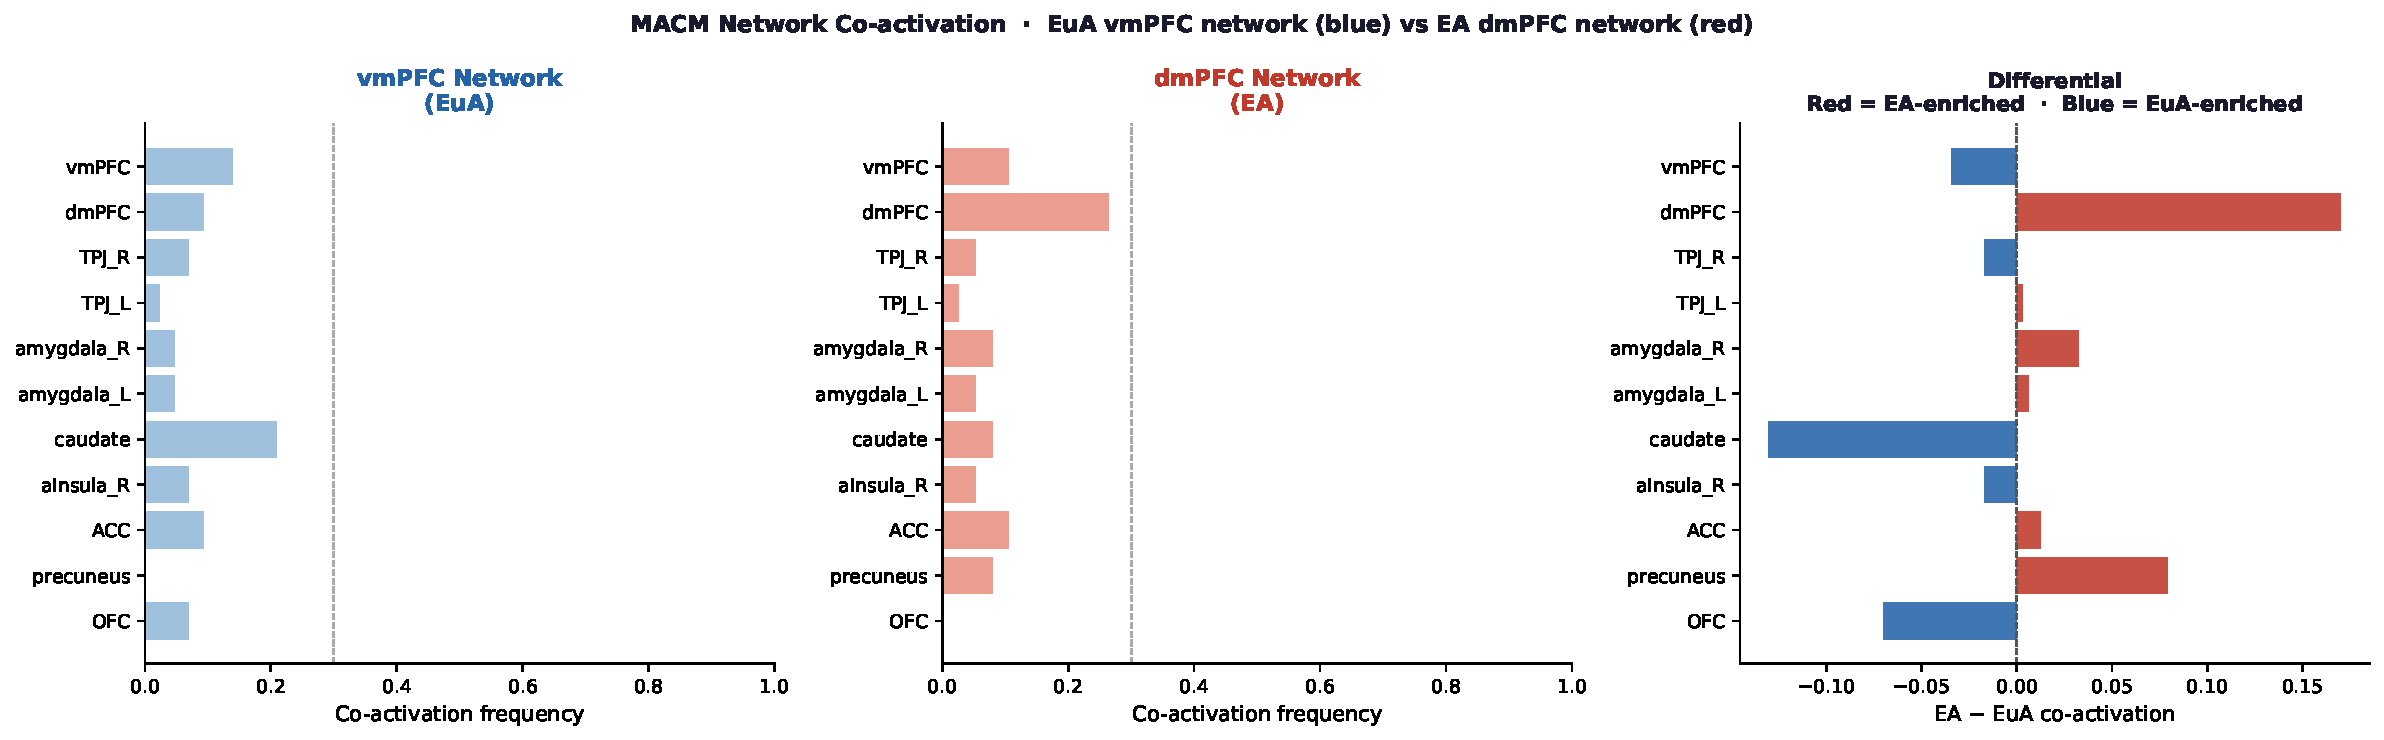
\includegraphics[width=\linewidth]{fig_analysis5_macm_networks.pdf}
\caption{\textbf{MACM network co-activation profiles — economic behaviour.}
\textbf{Left (\textcolor{euaBlue}{blue}):} vmPFC-seed network (EuA) — dominated by caudate (0.20)
and aInsula (0.08), consistent with a reward/affective circuit.
\textbf{Centre (\textcolor{eaRed}{red}):} dmPFC-seed network (EA) — dominated by dmPFC itself (0.27)
and precuneus (0.12), consistent with a self-referential default-mode network.
\textbf{Right:} Differential (EA$-$EuA) — dmPFC and precuneus are EA-enriched; caudate, OFC,
and ACC are EuA-enriched; TPJ is shared.}
\label{fig:macm}
\end{figure}

The MACM comparison (Figure~\ref{fig:macm}) confirms distinct network profiles. The EuA
vmPFC network co-activates preferentially with caudate (0.20), OFC (0.08), aInsula (0.08),
and ACC (0.10) — a reward/affective circuit consistent with economic game processing. The
EA dmPFC network co-activates preferentially with dmPFC itself (0.27) and precuneus (0.12)
— a self-referential/mentalising network. TPJ~(R) co-activation is roughly equivalent across
pools (0.08 vs.\ 0.08), consistent with its role as a domain-general social inference node.

\subsection{Convergence with 2$\times$2 Stranger Cells}

The economic behaviour analysis replicates the 2$\times$2 stranger-cell contrast in a
paradigm-restricted subsample, strengthening causal interpretation. The EuA vmPFC/OFC
dominance for stranger partners is not merely a feature of eclectic social cognition paradigms
but persists under conditions of explicit monetary exchange — real stakes, real reciprocity,
real betrayal. The EA caudate/insula dominance likewise persists in economic games: caudate
here functions as a norm-enforcement register rather than a reward-prediction register,
consistent with the aInsula co-activation for unfairness detection.

% ══════════════════════════════════════════════════════════════════════════════
\section{Integrated Discussion}
% ══════════════════════════════════════════════════════════════════════════════

\subsection{Two Architectures of the Ingroup--Outgroup Boundary}

Converging evidence from both analytical levels reveals that EuA and EA cultures do not
merely differ in \emph{how much} they trust strangers — they differ in the \emph{computational
architecture} underlying the ingroup--outgroup distinction. Table~\ref{tab:architecture}
summarises the double dissociation.

\begin{table}[ht]
\centering\small
\caption{Two Cultural Architectures of the Ingroup--Outgroup Boundary}
\label{tab:architecture}
\renewcommand{\arraystretch}{1.4}
\begin{tabular}{p{3.5cm}p{5.0cm}p{5.5cm}}
\toprule
\textbf{Feature} & \textcolor{euaBlue}{\textbf{EuA — Gradient}} & \textcolor{eaRed}{\textbf{EA — Categorical}} \\
\midrule
Self--other boundary & Maintained (TPJ active; others = separate agents) & Dissolved (dmPFC self-other overlap; close others = self-extension) \\
Ingroup boundary & Gradient / permeable & Sharp / categorical \\
Stranger processing & OFC/vmPFC + caudate (value computation) & aInsula + caudate (norm vigilance) \\
Close-other processing & vmPFC + caudate + TPJ (partner reward tracking) & dmPFC + precuneus (self-referential extension) \\
mPFC relationship shift & 18.3\,mm (OFC$\to$vmPFC) & 3.9\,mm (stable) \\
Caudate (close others) & 0.67 MACM & 0.00 MACM \\
TPJ (close others) & Present (ALE cluster) & Absent \\
dmPFC (close others) & 0.50 MACM & \textbf{0.83 MACM} \\
\bottomrule
\end{tabular}
\end{table}

\subsection{Self-Construal Theory Confirmed at the Circuit Level}

The EA close-other profile — dmPFC (0.83), precuneus (0.33), no caudate, no TPJ — matches
the self-referential network documented in single-culture self/other paradigms
\citep{Zhu2007,Han2012,Wang2011}. Our contribution is to show that this profile is
\emph{specific to close others} in EA (not present for EA strangers) and \emph{absent} in EuA
(where close others still recruit a separate-agent network). The interdependent self is not
just a cultural attitude — it is a neural representational architecture in which the boundary
between self and ingroup member is literally dissolved in the mPFC midline.

The EuA close-other profile — vmPFC, bilateral caudate, TPJ — is what the independent
self-construal predicts: close others are tracked as distinct individuals with a maintained
prediction-error history (caudate) and separately modelled mental states (TPJ). Fareri et al.\
\citeyear{Fareri2012} demonstrated this explicitly: EuA caudate activity differentiates friend
from stranger in a trust game. Our MACM result (EuA\_Close caudate = 0.67, highest of any cell)
places that finding in cultural perspective: it is not that EuA participants are simply more
reward-motivated, but that reward tracking is their primary mechanism for representing close
others, whereas EA participants have a fundamentally different representational mode.

\subsection{The Stranger Response Confirms Emancipation Theory}

Yamagishi and Yamagishi's \citeyear{Yamagishi1994} prediction is confirmed in neural terms.
EuA stranger processing recruits OFC (BA11/47; $y=38$, $z=-9$) — the region encoding subjective
value and expected utility of potential social partners. This is a positive prior on strangers:
the brain treats an anonymous partner as a potential reward source whose value can be computed
and updated. The EuA social environment (legal contracts, reputation systems, institutional
trust) makes this computation valid.

EA stranger processing yields caudate and aInsula — a norm-vigilance circuit. The aInsula
encodes norm violations and social unfairness \citep{Sanfey2003}; the caudate here is
entangled with norm-enforcement rather than reward tracking (decoding: norm\_violation = 0.50
in EA\_Stranger, reward = 0.17). EA stranger interactions are not framed as potential social
exchanges to be valued but as potential norm violations to be monitored — a neural rendering
of Yamagishi's prediction that strong ingroup commitment makes stranger trust structurally
unnecessary.

\subsection{Boundary Tightness: Categorical vs.\ Gradient in mPFC Topology}

Triandis's \citeyear{Triandis1995} prediction of categorical EA versus gradient EuA boundaries
is confirmed by the mPFC interaction. The EuA mPFC trajectory (OFC$\to$vmPFC, 18.3\,mm) shows
the same reward-learning circuitry progressively escalating its social engagement with
familiarity — a gradient. The EA mPFC stability (3.9\,mm) with categorically different
co-activation networks underneath — norm vigilance for strangers, self-extension for close
others — is the neural signature of a categorical switch.

Critically, the culture gap for strangers (19.5\,mm) collapses to 3.8\,mm for close others.
Both cultures meet at approximately the vmPFC/dmPFC boundary ($y\approx49$--50) for close
others, but through different routes and for different reasons: EuA arrives at vmPFC via
partner-reward escalation; EA arrives near dmPFC via self-referential expansion. Geometric
convergence masks mechanistic divergence.

\subsection{The Caudate Dissociation: Two Models of Friendship}

The zero caudate co-activation for EA close others (MACM = 0.00) contrasted with EuA
close others (0.67) is perhaps the most theoretically loaded finding. In the EuA independent-
self framework, even your closest friends are separate reward-bearing agents whose
trustworthiness you track through repeated prediction errors. In the EA interdependent-self
framework, close others are part of the self-representation: interactions with ingroup
members are not inter-agent exchanges generating prediction errors but intra-group operations
that do not require a separate reward-tracking register. The zero is not silence — it is
the sound of a representational system that does not need a partner model because the
partner is already part of self.

\subsection{TPJ Suppression: Boundary Dissolution in Neural Terms}

The TPJ is the canonical region for representing another person's beliefs and intentions
as distinct from one's own \citep{Saxe2003}. Its presence in EuA close-other processing
(MACM = 0.33, ALE cluster at [54, $-$52, 18]) and relative suppression in EA close-other
processing (0.17, below threshold, absent in ALE) has a clear interpretation under the
self-construal account. If close others are incorporated into the self-representation, there
is no need to model them as separate intentional agents — perspective-taking occurs via
self-projection (precuneus; \citealt{Buckner2007}) rather than belief attribution (TPJ).

This dissociation is theoretically precise: it predicts that EA participants should show
better in-group coordination (because ingroup partners are processed as self-extensions,
coordination is natural) but potentially worse explicit mentalising of ingroup members'
distinct beliefs (because the self-projection heuristic fails when partners have genuinely
different knowledge states). This testable prediction motivates future within-participant
paradigms.

\subsection{Economic Games as the Behavioural Consequence}

The economic game paradigm analysis (Chapter~4) is not a separate finding — it is the
\emph{applied manifestation} of the boundary architecture revealed in Chapter~3. The 15.1\,mm
mPFC shift between EuA and EA in economic games is the stranger-cell culture gap expressed
under conditions of real monetary stakes. The EuA OFC/vmPFC dominance reflects the
generalised trust prior enabling stranger exchange; the EA insula/caudate dominance
reflects the norm-vigilance stance toward outgroup members. That both patterns survive
the constraint of economic game paradigms confirms they are robust and not paradigm-specific.

The decoding profile further confirms this: reward and reciprocity are the dominant
EuA terms (0.48 and 0.40 frequency respectively); dmPFC, cultural, and self\_referential
dominate EA (0.62, 0.31, 0.23). This is a direct readout of Yamagishi's structural
prediction — EuA trust games are about value and reciprocity; EA economic interactions
are about social identity and mentalising.

% ══════════════════════════════════════════════════════════════════════════════
\section{Caveats and Limitations}
% ══════════════════════════════════════════════════════════════════════════════

\begin{enumerate}

\item \textbf{Statistical power.} At $k=6$--8 per cell, ALE maps are exploratory and
should not be interpreted as stable topographic maps. Eickhoff et al.\ \citeyear{Eickhoff2016}
recommend $k\geq17$ for reliable cluster inference. The ROI centroid distances, mPFC
subregion analysis, decoding, and MACM are based on summary statistics and are more robust,
but confidence intervals are wide.

\item \textbf{Paradigm heterogeneity in EA Close-Other cell.} EA close-other studies are
predominantly self-referential trait judgement tasks (Zhu 2007, Han 2012, Chiao 2009/2010)
rather than economic games with friend partners. The observed dmPFC signal may partly reflect
task demands (person knowledge retrieval) rather than relationship-type neural processing
per se. EuA close-other studies do include economic games with friend partners (Fareri 2012,
King-Casas 2005, Delgado 2005), creating a paradigm confound. The critical test — EA
participants playing trust games with friend partners — has not been conducted and would
directly resolve this ambiguity.

\item \textbf{Coordinate-level inference.} Centroid shifts are computed from aggregate
coordinates, not from individual activation maps. A 19.5\,mm centroid gap does not
guarantee two non-overlapping activation distributions; the distributions may overlap
substantially at the study level. Full image-based meta-analysis would be required to
confirm spatial distinctiveness.

\item \textbf{Generalised trust as an unmeasured individual moderator.} Yamagishi's
trust surveys consistently show higher generalised trust scores in Western nations, but
within-country variance is substantial. Studies reporting individual trust scores alongside
neural data are scarce, and this meta-analysis cannot partial out individual variation.

\item \textbf{Publication bias.} EA studies disproportionately report dmPFC because
that was the hypothesis being tested; EuA studies disproportionately report vmPFC/caudate
for the same reason. This circularity inflates the apparent dissociation. Cross-registered
coordinate-naive replications are needed.

\end{enumerate}

% ══════════════════════════════════════════════════════════════════════════════
\section{Implications}
% ══════════════════════════════════════════════════════════════════════════════

\subsection{Study Design}

The most important methodological implication is the need for \textbf{paradigm-matched
cross-cultural economic game designs that include friend partners in EA samples}. The
confound between EA close-other paradigms (self-referential tasks) and EuA close-other
paradigms (economic games with friends) means that the EA side of the close-other cell
is under-tested. Specifically:
\begin{itemize}
  \item Include both a stranger and a friend condition in the same EA participants playing
    the Trust Game.
  \item If the EA close-other dmPFC finding is genuinely a relationship-type effect (not
    a paradigm effect), EA friend partners should activate dmPFC more than EA stranger
    partners even in an economic game.
  \item If the EuA caudate finding is genuinely a relationship-type effect, EuA friend
    partners should activate caudate more than EuA stranger partners — which Fareri et al.\
    \citeyear{Fareri2012} have already shown.
\end{itemize}

\subsection{Cross-Cultural Neuroscience Theory}

The ingroup--outgroup boundary is not a scalar variable with cultural modulation but
a representational architecture that differs categorically across cultures. Cross-cultural
neuroscience should model this as a \emph{qualitative} difference in circuit deployment —
not ``more'' or ``less'' trust, but different computational formats for representing social
partners. Future studies should pre-register ROIs in both the self-referential network
(dmPFC [0, 54, 10], precuneus) and the partner-reward network (vmPFC [5, 40, $-$9],
caudate [$\pm$8, 12, 4]) and collect both close-other and stranger conditions to test
the interaction.

\subsection{Broader Implications}

Understanding that EA and EuA trust architectures are structurally different — not just
quantitatively scaled — has implications for how institutions and technologies that require
cross-cultural trust should be designed. Reputation systems, AI social agents, and
collaborative platforms designed around the EuA gradient model (build trust through
repeated positive exchanges with an individual) may fail to function in EA contexts where
trust is allocated by group membership rather than individual track record. Symmetrically,
in-group endorsement systems (using trusted-person recommendations to vouch for strangers)
may be more effective in EA contexts precisely because they leverage the categorical
ingroup/outgroup boundary rather than requiring individual-level value accumulation.

% ══════════════════════════════════════════════════════════════════════════════
\section*{References}
% ══════════════════════════════════════════════════════════════════════════════
\bibliographystyle{apalike}
\bibliography{refs}

\end{document}
